%-----------------------------------------------------------------------
% Beginning of chap2.tex
%-----------------------------------------------------------------------
%
%  AMS-LaTeX sample file for a chapter of a monograph, to be used with
%  an AMS monograph document class.  This is a data file input by
%  chapter.tex.
%
%  Use this file as a model for a chapter; DO NOT START BY removing its
%  contents and filling in your own text.
% 
%%%%%%%%%%%%%%%%%%%%%%%%%%%%%%%%%%%%%%%%%%%%%%%%%%%%%%%%%%%%%%%%%%%%%%%%


\chapter*{Lecture 3}
\addcontentsline{toc}{chapter}{Lecture 3}
\setcounter{chapter}{3}
\setcounter{equation}{0}
\setcounter{theorem}{0}
\setcounter{section}{0}
%\numberwithin{section}{chapter}
\numberwithin{equation}{chapter}
\numberwithin{theorem}{chapter}
% \epigraph{}{--- \textup{}}

Most modern optimization methods are iterative: they generate a sequence of points $\vct{x}_0,\vct{x}_1,\dots$ in $\R^n$
in the hope that this sequences will converge to a local or global minimizer $\vct{x}^*$ of a function $f(\vct{x})$. A typical rule for generating such a sequence would be to start with a vector $\vct{x}_0$, chosen by an educated guess, and then for $k\geq 0$, move from step $k$ to $k+1$ by
\begin{equation*}
 \vct{x}_{k+1} = \vct{x}_k+\alpha_k\vct{p}_k,
\end{equation*}
in a way that ensures that $f(\vct{x}_{k+1})\leq f(\vct{x}_k)$.
The parameter $\alpha_k$ is called the \textbf{step length}, while $\vct{p}_k$ is the \textbf{search direction}. In this lecture we discuss one such method, the method of gradient descent, or steepest descent, and discuss how to select the right step length.

\section{Gradient descent} 
In the method of gradient descent, the search direction is chosen as
\begin{equation}\label{eq:gradient}
 \vct{p}_k = -\nabla f(\vct{x}_k).
\end{equation}
To see why this makes sense, let $\vct{p}$ be a direction and consider the Taylor expansion
\begin{equation*}
 f(\vct{x}_k+\alpha \vct{p}) = f(\vct{x}_k)+\alpha \ip{\vct{p}}{\nabla f(\vct{x}_k)}+O(\alpha^2).
\end{equation*}
Considering this as a function of $\alpha$, the rate of change in direction $\vct{p}$ at $\vct{x}_k$ is the derivative of this function at $\alpha=0$,
\begin{equation*}
 \frac{\diff{f}(\vct{x}_k+\alpha \vct{p})}{\diff{\alpha}}|_{\alpha=0} = \ip{\vct{p}}{\nabla f(\vct{x}_k)},
\end{equation*}
also known as the \textbf{directional derivative} of $f$ at $\vct{x}_k$ in the direction $\vct{p}$.
This formula indicates that the rate of change is {\em negative}, and we have a \textbf{descent direction}, if $\ip{\vct{p}}{\nabla f(\vct{x}_k)}<0$. 

The Cauchy-Schwarz inequality (see Preliminaries, Page 9) gives the bounds
\begin{equation*}
 -\norm{\vct{p}}_2 \norm{\nabla f(\vct{x}_k)}_2 \leq \ip{\vct{p}}{\nabla f(\vct{x}_k)} \leq \norm{\vct{p}}_2 \norm{\nabla f(\vct{x}_k)}_2.
\end{equation*}
We see that the rate of change is the smallest when the first inequality is an equality, which happens if 
\begin{equation*}
 \vct{p} = -\alpha \nabla f(\vct{x}_k)
\end{equation*}
for some $\alpha>0$. 

For a visual interpretation of what it means to be a descent direction, note that the \textbf{angle} $\theta$ between a vector $\vct{p}$ and the gradient $\nabla f(\vct{x})$ at a point $\vct{x}$ is given by (see Preliminaries, Page 9)
\begin{equation*}
  \ip{\vct{x}}{\nabla f(\vct{x})} = \norm{\vct{p}}_2\norm{\nabla f(\vct{x})}_2 \cos(\theta).
\end{equation*}
This is negative if the vector $\vct{p}$ forms and angle greater than $\pi/2$ with the gradient. Recall that the gradient points in the direction of steepest ascent, and is orthogonal to the {\em level sets}. If you are standing on the slope of a mountain, walking along the level set lines will not change your elevation, the gradient points to the steepest upward direction, and the negative gradient to the steepest descent.

\begin{figure}[h!]
\centering
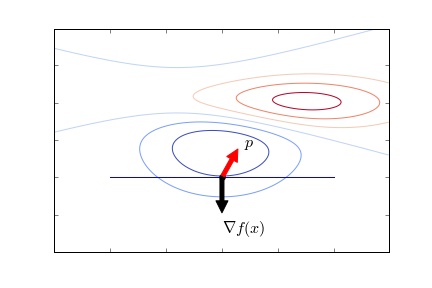
\includegraphics[width=0.6\textwidth]{images/descent.png}
\caption{A descent direction}
\end{figure}

Any multiple $\alpha \nabla f(\vct{x}_k)$ points in the direction of steepest descent, but we have to choose a sensible parameter $\alpha$ to ensure that we make sufficient progress, but at the same time don't overshoot. Ideally, we would choose the value $\alpha_k$ that minimizes $f(\vct{x}_k-\alpha_k \nabla f(\vct{x}_k))$. While finding such a minimizer is in general not easy (see Section Lecture 4 for alternatives), for quadratic functions in can be given in closed form.

\subsection{Linear least squares} Consider a function of the form
\begin{equation*}
 f(\vct{x}) = \frac{1}{2}\norm{\mtx{A}\vct{x}-\vct{b}}_2^2.
\end{equation*}
In Problem Sheet 1 you will show that that the Hessian is symmetric and positive semidefinite, with the gradient given by
\begin{equation*}
 \nabla f(\vct{x}) = \mtx{A}^{\trans}(\mtx{A}\vct{x}-\vct{b}).
\end{equation*}
The method of gradient descent proceeds as
\begin{equation*}
 \vct{x}_{k+1} = \vct{x}_k-\alpha_k \mtx{A}^{\top}(\mtx{A}\vct{x}_k-\vct{b}).
\end{equation*}
To find the best $\alpha_k$, we compute the minimum of the function
\begin{equation}\label{eq:minalpha}
 \alpha \mapsto f(\vct{x}_k-\alpha \mtx{A}^{\trans}(\mtx{A}\vct{x}_k-\vct{b})).
\end{equation}
If we set $\vct{r}_k:=\mtx{A}^{\trans}(\vct{b}-\mtx{A}\vct{x}_k) = -\nabla f(\vct{x}_k)$ and compute the minimum of~\eqref{eq:minalpha} by differentiating, we get the step length
\begin{equation*}
 \alpha_k = \frac{\vct{r}_k^{\trans}\vct{r}_k}{\vct{r}_k^{\trans}\mtx{A}^\trans\mtx{A}\vct{r}_k} = \frac{\norm{\vct{r}_k}_2^2}{\norm{\mtx{A}\vct{r}_k}_2^2}.
\end{equation*}
(Verify this!) Note also that when we have $\vct{r}_k$ and $\alpha_k$, we can compute the next $\vct{r}_k$ as
\begin{align*}
 r_{k+1} &= \mtx{A}^{\trans}(\vct{b}-\mtx{A}\vct{x}_{k+1})\\
         &= \mtx{A}^{\trans}(\vct{b}-\mtx{A}(\vct{x}_{k}+\alpha_k \vct{r}_k))\\
         &= \mtx{A}^{\trans}(\vct{b}-\mtx{A}\vct{x}_k - \alpha_k \mtx{A}^{\trans}\mtx{A}\vct{r}_k) = \vct{r}_k - \alpha_k \mtx{A}^{\trans}\mtx{A}\vct{r}_k.
\end{align*}
The gradient descent algorithm for the linear least squares problem proceeds by first computing $\vct{r}_0=\mtx{A}^{\trans}(\vct{b}-\mtx{A}\vct{x}_0)$, and then at each step
\begin{align*}
 \alpha_k &= \frac{\vct{r}_k^{\trans}\vct{r}_k}{\vct{r}_k^{\trans}\mtx{A}^\trans\mtx{A}\vct{r}_k}\\
 \vct{x}_{k+1} &= \vct{x}_k+\alpha_k \vct{r}_k\\
 \vct{r}_{k+1} &= \vct{r}_k - \alpha_{k}\mtx{A}^{\trans}\mtx{A}\vct{r}_k.
\end{align*}
Does this work? How do we know when to stop? It is worth noting that the residual satisfies $\vct{r}=0$ if and only if $\vct{x}$ is a stationary point, in our case, a minimizer. One criteria for stopping could then be to check whether $\norm{\vct{r}_k}_2\leq \e$ for some given tolerance $\e>0$. One potential problem with this criterion is that the function can become {\em flat} long before reaching a minimum, so an alternative stopping method would be to stop when the difference between two successive points, $\norm{\vct{x}_{k+1}-\vct{x}_k}_2$, becomes smaller than some $\e>0$.

\begin{example}
We plot the trajectory of gradient descent with the data

\begin{figure}[h!]
\centering
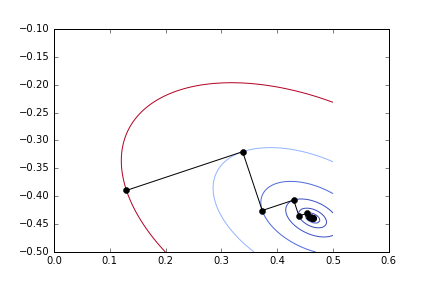
\includegraphics[width=0.5\textwidth]{images/graddescent.png}
\caption{Trajectory of gradient descent}
\end{figure}

\begin{equation*}
\mtx{A} = \begin{pmatrix}
2 & 0\\
1 & 3\\
0 & 1
\end{pmatrix}, \quad
\vct{b} = \begin{pmatrix}
1\\ -1\\ 0
\end{pmatrix}.
\end{equation*}


As can be seen from the plot, we always move in the direction orthogonal to a level set, and stop at a point where we are tangent to a level set.
\end{example}



%-----------------------------------------------------------------------
% End of chap1.tex
%-----------------------------------------------------------------------
